%  !TeX  root  =  user_guide.tex

\chapter{Lavorare con le proiezioni}\label{label_projections}
\index{Projections!working with}

% when the revision of a section has been finalized,
% comment out the following line:
%\updatedisclaimer

QGIS consente all'utente di definire un sistema di riferimento - SR - (Coordinate Reference System, ovvero Sistema 
di Riferimento delle Coordinate) globale o a livello di singolo progetto per i layer privi di un SR predefinito. 
Consente inoltre di definire sistemi di coordinate personalizzati e supporta la riproiezione al volo (on-the-fly, OTF) 
dei layer vettoriali. Tutte queste caratteristiche permettono all'utente di visualizzare contemporaneamente 
e correttamente sovrapposti layer aventi SR differenti

\section{Panoramica sul supporto alle proiezioni}\label{label_projoverview}

QGIS supporta all'incirca 2.700 SR. Le definizioni di ognuno di questi SR sono memorizzate in un database SQLite 
che viene installato con QGIS. Normalmente non è necessario manipolare il database direttamente, infatti questa operazione 
può causare il malfunzionamento del supporto alla proiezione. I SR personalizzati sono salvati in un database utente.
Si veda la Sezione \ref{sec:customprojections} per informazioni sulla gestione dei SR personalizzati.

I SR disponibili in QGIS sono basati su quelli definiti dall'European Petroleum Survey Group - EPSG\index{EPSG} - e 
dall'Institut Geographique National francese (IGN)\index{IGN} e sono per lo più tratti dalle tabelle di riferimento 
spaziale di GDAL\index{GDAL}. Gli identificatori EPSG sono presenti nel database e possono essere usati per 
richiamare e definire i SR in QGIS.

Per usare la riproiezione al volo (OTF), i dati devono contenere informazioni sul proprio sistema di riferimento 
oppure bisogna definire un SR a livello layer o a livello di progetto o globale. Per i layer PostGIS, 
QGIS usa l'identificatore del riferimento spaziale specificato al momento della creazione del layer.
Per i dati supportati da OGR, QGIS fa affidamento sulla presenza di un mezzo, specifico per ciascun formato, 
che definisce il SR. Nel caso degli shapefile, ad esempio, si stratta di un file contenente l'indicazione del SR 
in formato Well Known Text (WKT)\index{WKT}. Il file della proiezione ha lo stesso nome dello shapefile, ma 
ha estensione prj. Per esempio uno shapefile chiamato \filename{alaska.shp} avrà un corrispondente file 
di proiezione chiamato \filename{alaska.prj}.

Ogni volta che si seleziona un nuovo SR, le unità utilizzate per il layer verranno automaticamente aggiornate 
nella scheda \tab{Generale} della finestra di dialogo \dropmenuopttwo{mActionOptions}{Proprietà Progetto} 
sotto il menu \mainmenuopt{Modifica} (Gnome, OS X) o \mainmenuopt{Impostazioni} (KDE, Windows).

\section{Specificare una proiezione}
\index{Proiezioni!specificare}
\label{sec:projection-specifying}

\begin{figure}[ht]
   \centering
   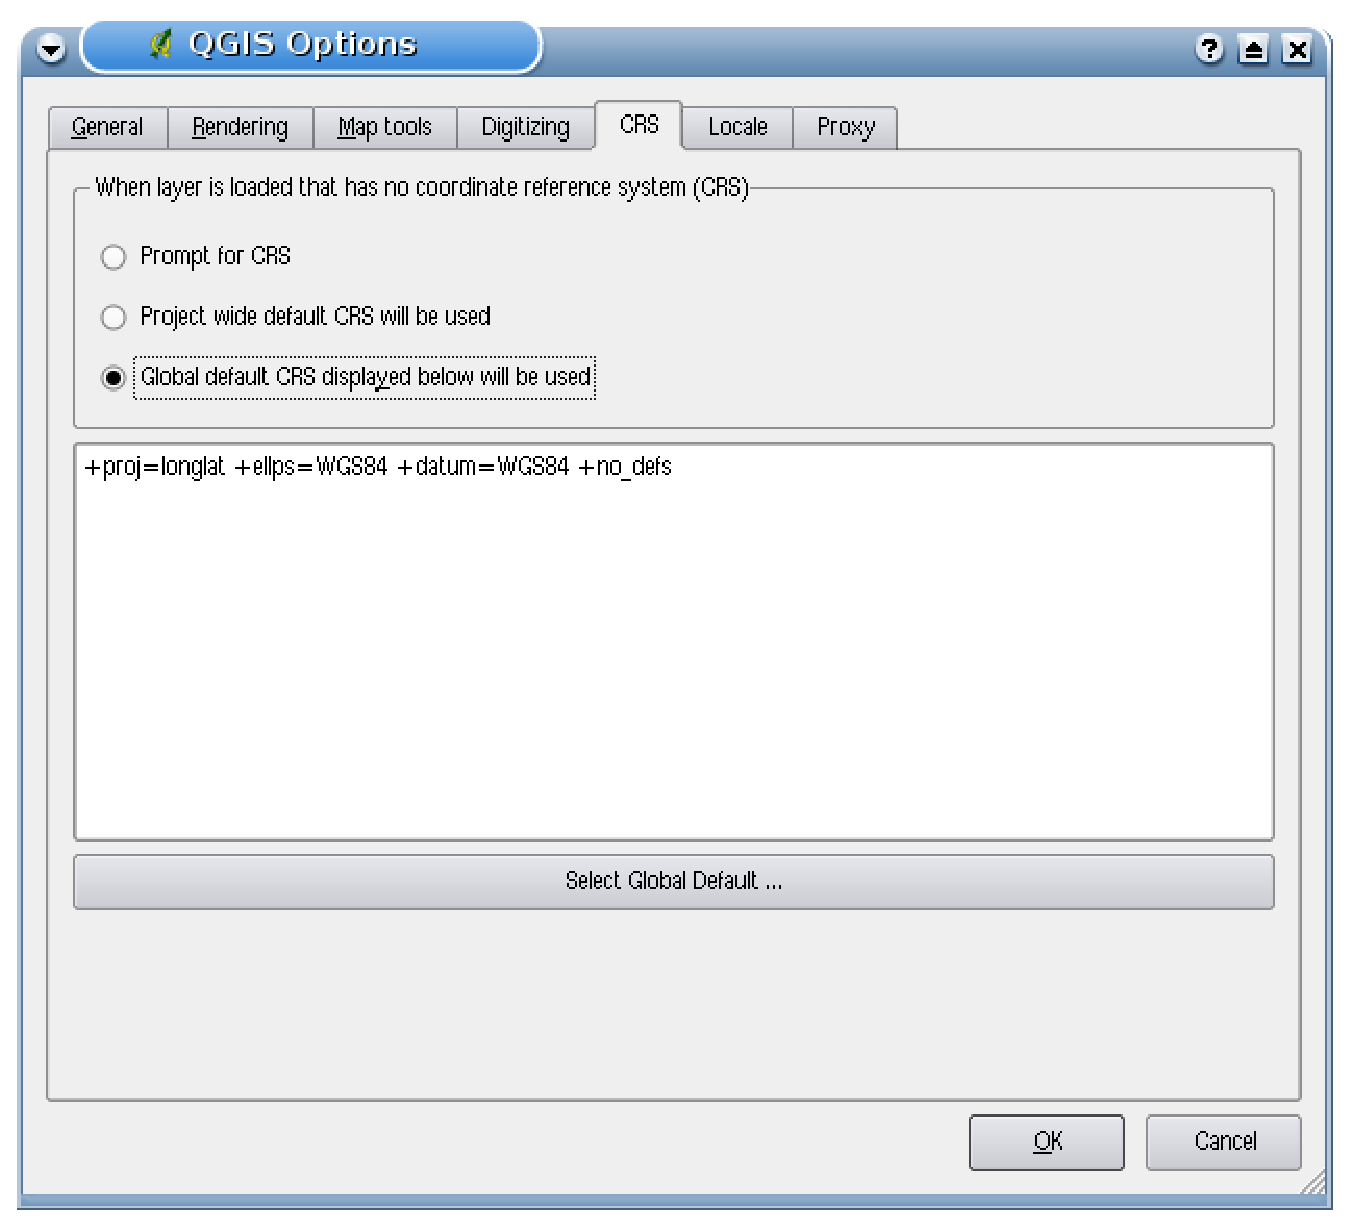
\includegraphics[clip=true, width=12cm]{crsdialog}
   \caption{Scheda SR nella finestra opzioni di QGIS \nixcaption}\label{fig:crsdialog}
\end{figure}

QGIS imposta il SR di ogni nuovo progetto su quello definito a livello globale: il SR globale predefinito è 
EPSG:4326 - WGS 84 (\texttt{proj=longlat +ellps=WGS84 +datum=WGS84 +no\_defs}). Il SR predefinito può essere 
modificato tramite il pulsante \button{Scegli...} mostrato in Figura~\ref{fig:crsdialog}: tale impostazione 
varrà per tutte le sessioni successive di QGIS.

Quando si utilizzano layer privi di SR, è necessario definire la risposta di QGIS a tale situazione.
Questo può essere fatto globalmente o a livello di progetto nella scheda \tab{SR} 
sotto la voce di menu \mainmenuopt{Modifica} \arrow \dropmenuopttwo{mActionOptions}{Opzioni} (Gnome, OSX) o
\mainmenuopt{Impostazioni} \arrow \dropmenuopttwo{mActionOptions}{Opzioni}(KDE, Windows).

Le opzioni mostrate in Figura~\ref{fig:crsdialog} sono:
\begin{itemize}[label=--]
\item \checkbox{Richiedi SR}
\item \checkbox{Usa il SR del progetto}
\item \checkbox{Utilizza come predefinito SR visualizzato sotto}
\end{itemize}

Per definire il SR di un layer privo di tale informazione, si può anche agire nella scheda \tab{Generale}
della finestra di dialogo delle proprietà dei raster (Sezione \ref{label_generaltab}) e dei vettori (Sezione \ref{vectorgeneraltab}). 
Se il SR è già stato definito, lo stesso verrà mostrato come nella Figura ~\ref{fig:vector_symbology}.

\begin{Tip}
\caption{\textsc{SR nella legenda}} Il menu contestuale dei layer in legenda (tasto destro sul nome del layer) 
(Sezione \ref{label_legend}) fornisce due scorciatoie per l'impostazione del SR:
\begin{itemize}
\item \dropmenuopt{Imposta il SR del layer}, che apre la finestra di dialogo Selettore sistema di riferimento (SR). 
La stessa finestra può essere raggiunta con il pulsante \button{Specifica...} nella scheda \button{Generale} delle proprietà del layer.
\item \dropmenuopt{Imposta il SR del progetto dal layer}, che imposta il SR del progetto sulla base di quello del layer.
\end{itemize}
\end{Tip}

\section{Definire la riproiezione al volo (OTF)}\label{label_projstart}

La nuova versione di QGIS supporta la riproiezione al volo (OTF) sia per i raster che per i vettori, ma l'opzione non 
è abilitata di default. Per usare la riproiezione OTF, bisogna attivare la casella di controllo 
\checkbox{Abilita la riproiezione al volo} nella scheda \tab{SR} della finestra di dialogo 
\dropmenuopttwo{mActionOptions}{Proprietà del progetto}.

Ci sono tre modi per aprire questa finestra:

\begin{enumerate}
\item Selezionare \dropmenuopttwo{mActionOptions}{Proprietà progetto} dal menu
\mainmenuopt{Modifica} (Gnome, OSX) o \mainmenuopt{Impostazioni} (KDE, Windows).
\item Fare click sull'icona \toolbtntwo{mIconProjectionDisabled}{Stato SR} nell'angolo 
in basso a destra della barra di stato.
\item Impostare la riproiezione in modalità predefinita attivando la casella di controllo 
\checkbox{Effettua sempre la riproiezione al volo} nella scheda \tab{SR} della finestra di 
dialogo \dialog{Opzioni}.
\end{enumerate}

Se è già stato caricato un layer e si vuole abilitare la riproiezione, è buona norma aprire
la scheda \tab{Sistema di riferimento (SR)} della finestra di dialogo 
\dialog{Proprietà del progetto} selezionare nell'elenco il SR attualmente impostato, 
quindi attivare la casella di controllo \checkbox{Abilita la riproiezione al volo}.
Ogni layer caricato successivamente sarà riproiettato al volo nel SR mostrato affianco al
pulsante \toolbtntwo{mIconProjectionEnabled}{Stato SR}.

La scheda \tab{Sistema di riferimento (SR)}) della finestra di dialogo \dialog{Proprietà del progetto}
contiene cinque importanti componenti, illustrati in Figura \ref{fig:projections} e di seguito descritti.

\begin{figure}[ht]
   \centering
   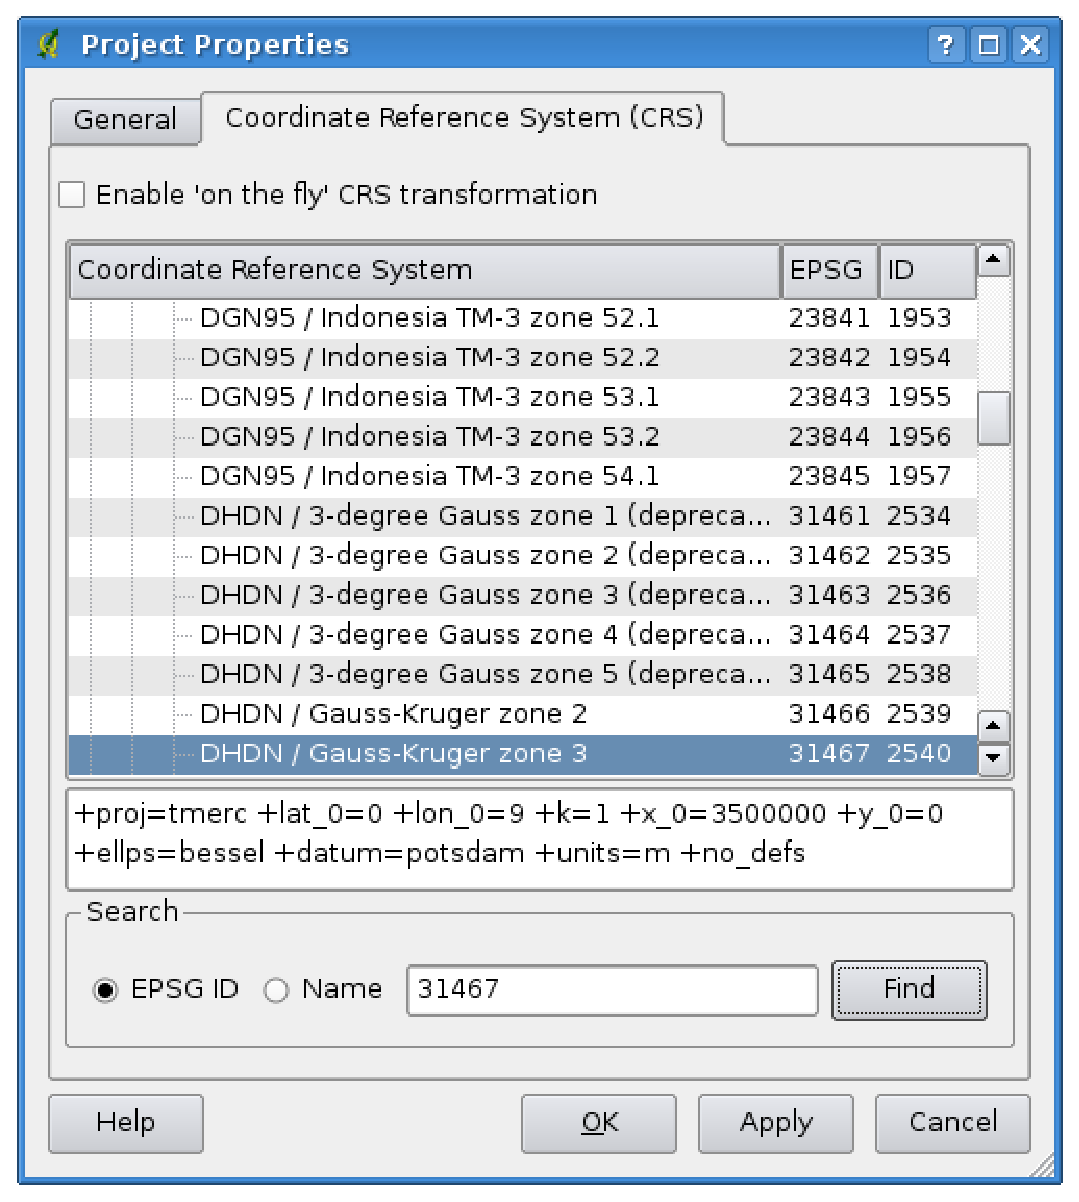
\includegraphics[clip=true, width=10cm]{projectionDialog}
   \caption{Finestra di dialogo per l'impostazione della proiezione \nixcaption}\label{fig:projections}
\end{figure}

\begin{enumerate}
\item \textbf{Abilita la riproiezione al volo}\index{Proiezioni!abilitare} -
questa casella di controllo è usata per attivare o disattivare la riproiezione al volo. 
Quando è deselezionata, ogni layer è tracciato usando le coordinate lette dal dato sorgente. 
Se abilitata, le coordinate di ogni layer sono riproiettate nel SR definito per la vista mappa.
\item \textbf{Sistema di Riferimento} - è la lista di tutti i SR supportati da QGIS, inclusi i
sistemi di coordinate geografiche, piane e quelli personalizzati. Per usare un SR, selezionarlo
dalla lista espandendo il gruppo appropriato. Il SR attivo è quello preselezionato.
\item \textbf{Stringa Proj4} - è la stringa SR usata dal motore di proiezione Proj4. 
È un testo di sola lettura, a solo scopo informativo.
\item \textbf{Cerca} - se si conosce il codice EPSG, l'identificatore o il nome del SR che si vuole impostare, 
può essere usata questa area di ricerca per trovarlo nell'elenco, inserendo una voce di ricerca e facendo click 
su \button{Trova}. Usare la casella \checkbox{Nascondi i SR sconsigliati} per mostrare solo le proiezioni attualmente approvate.
\item \textbf{Sistemi di riferimento usati di recente} - se ci sono dei SR che vengono usati frequentemente, 
essi verranno visualizzati in questa sezione della finestra di dialogo. Basta fare click su una voce per impostare il SR associato.
\end{enumerate}

\begin{Tip}
\caption{\textsc{Finestra di dialogo Proprietà del progetto}}
Se si apre la finestra di dialogo \dialog{Proprietà del progetto} dal menu \mainmenuopt{Modifica} (Gnome, OSX) 
o \mainmenuopt{Impostazioni} (KDE, Windows), bisogna fare click sulla scheda \tab{Sistema di 
riferimento (SR)} per visualizzare le impostazioni del SR. La stessa finestra può essere aperta con 
l'icona \toolbtntwo{mIconProjectionEnabled}{Stato SR}.
\end{Tip}

\section{Sistemi di riferimento personalizzati}\label{sec:customprojections}
\index{Proiezioni!personalizzare}

Se in QGIS non si trova il sistema di riferimento di cui si necessita, 
è possibile definirne uno personalizzato: selezionare \dropmenuopttwo{mIconNew}{SR personalizzato} 
dal menu \mainmenuopt{Modifica} (Gnome, OSX) o \mainmenuopt{Impostazioni} (KDE, Windows). 
I SR personalizzati sono salvati nel database utente di QGIS. Oltre ai SR personalizzati, 
questo database contiene anche i segnalibri geospaziali e altri dati personalizzati dall'utente.

\begin{figure}[ht]
   \centering
   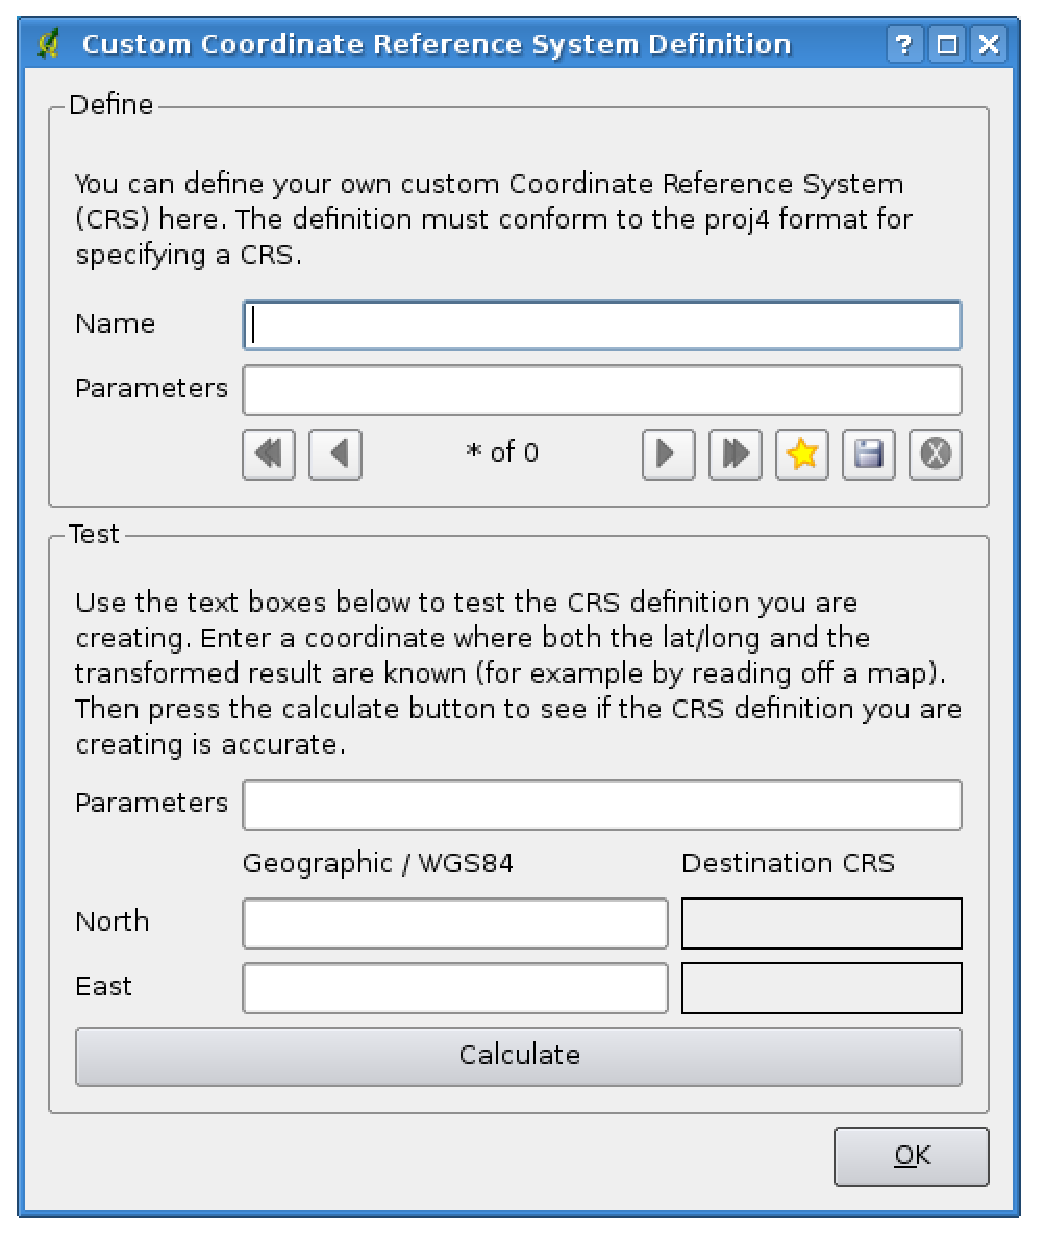
\includegraphics[clip=true, width=8cm]{customProjectionDialog}
   \caption{Finestra di dialogo per i SR personalizzati \nixcaption}\label{fig:customprojections}
\end{figure}

La definizione di un SR personalizzato in QGIS richiede una buona comprensione delle librerie
Proj.4. Per iniziare, fare riferimento al documento "Cartographic Projection Procedures for the UNIX Environment - A User's Manual" di Gerald I. Evenden, U.S. Geological Survey Open-File Report 90-284, 1990 
(disponibile all'indirizzo \url{ftp://ftp.remotesensing.org/proj/OF90-284.pdf}). 
Questo manuale descrive l'uso di \usertext{proj.4} e delle relative utilità da riga di comando. 
I parametri cartografici usati da \usertext{proj.4} sono descritti nel manuale e sono identici a quelli usati da QGIS.

La finestra di dialogo \dialog{Definizione Sistema Riferimento Spaziale Personalizzato} richiede solo due
parametri per definire un SR personalizzato:
\begin{enumerate}
\item un nome descrittivo e
\item i parametri cartografici in formato PROJ.4.
\end{enumerate}
Per creare un nuovo SR, fare click sul pulsante \toolbtntwo{mIconNew}{Nuovo} e inserire 
il nome descrittivo e i parametri. Successivamente salvare il SR facendo click sul pulsante \toolbtntwo{mActionFileSave}{Salva}.

Si noti che la voce \guilabel{Parametri} deve iniziare con un blocco \usertext{+proj=}, per rappresentare il nuovo SR.

È possibile testare i parametri SR per vedere se danno risultati validi facendo click sul pulsante
\button{Calcola} nella sezione \guiheading{Prova}, dopo aver incollato i parametri SR personalizzati 
nel campo \guilabel{Parametri}.
Quindi, inserire dei valori noti di latitudine e longitudine nel sistema WGS 84 rispettivamente nei campi 
\guilabel{Nord} e \guilabel{Est}. 
Fare click su \button{Calcola} e confrontare i risultati con i valori noti nel SR personalizzato.

\FloatBarrier
